\documentclass[11pt,a4paper]{article}

%================ PACKAGES ==================
\usepackage[T1]{fontenc}
\usepackage{lmodern}
\usepackage[a4paper,margin=1in]{geometry}
\usepackage{graphicx}
\usepackage{titlesec}
\usepackage{setspace}
\usepackage{amsmath}
\usepackage{amssymb}
\usepackage{booktabs}
\usepackage{float}
\usepackage{caption}
\usepackage{array}
\usepackage{fancyhdr}
\usepackage{xcolor}
\usepackage{colortbl}
\usepackage{hyperref}
\usepackage{lastpage}
\usepackage{refcount}
\usepackage[backend=biber,style=ieee,sorting=none]{biblatex}
\usepackage{enumitem}
\usepackage{tikz}
\usepackage{pgfplots}
\usepackage[skins,breakable]{tcolorbox}
\usepackage{microtype}
\usetikzlibrary{arrows.meta,positioning,shadows.blur,shapes.geometric,calc,fit,backgrounds}
\pgfplotsset{compat=1.18}
\addbibresource{references.bib}

%================ COLOR THEME ==================
\definecolor{prismblue}{HTML}{173B73}
\definecolor{prismcyan}{HTML}{2AA7B8}
\definecolor{prismlight}{HTML}{EAF6F8}
\definecolor{prismgold}{HTML}{F2B705}
\definecolor{prismgray}{HTML}{4D5B6A}
\definecolor{prismnavy}{HTML}{0B1F3A}
\definecolor{prismgreen}{HTML}{2E8B57}
\definecolor{prismred}{HTML}{C94C4C}

\hypersetup{
    colorlinks=true,
    linkcolor=prismblue,
    urlcolor=prismcyan,
    citecolor=prismblue
}

\setlist[itemize]{leftmargin=1.4cm,label=\textcolor{prismcyan}{\small$\blacktriangleright$}}
\setlist[enumerate]{leftmargin=1.4cm,label=\textcolor{prismblue}{\bfseries\arabic*.}}

%================ PROFESSIONAL BOXES ==================
\tcbset{
    enhanced,
    boxrule=0pt,
    arc=3mm,
    left=4mm,
    right=4mm,
    top=3mm,
    bottom=3mm,
    fonttitle=\bfseries,
    coltitle=white,
    drop fuzzy shadow
}

\newtcolorbox{summarybox}[1]{
    colback=prismlight,
    colframe=prismblue,
    borderline west={2pt}{0pt}{prismcyan},
    title=#1,
    colbacktitle=prismblue
}

\newcommand{\metriccard}[3]{%
\begin{tikzpicture}[baseline=(box.base)]
    \node[rounded corners=6pt,fill=#1!12,draw=#1!65,line width=0.6pt,minimum width=3.6cm,minimum height=1.45cm,align=center,blur shadow] (box) {\textcolor{#1}{\Large\bfseries #2}\\[-1mm]{\scriptsize\textcolor{prismgray}{#3}}};
\end{tikzpicture}%
}

\newcommand{\reportprogress}{%
\begin{tikzpicture}[baseline=-0.45ex]
    \pgfmathsetmacro{\documentprogress}{min(1,max(0,\value{page}/max(1,\getpagerefnumber{LastPage})))}
    \fill[prismgray!22,rounded corners=0.5pt] (0,0) rectangle (2.6,0.055);
    \fill[prismcyan,rounded corners=0.5pt] (0,0) rectangle ({2.6*\documentprogress},0.055);
\end{tikzpicture}%
}

\newcommand{\termrow}[2]{\textbf{#1} & #2 \\}


%================ FONT SETTINGS ==================
\renewcommand{\familydefault}{\rmdefault}

%================ SPACING ==================
\singlespacing

%================ CAPTION SETTINGS ==================
\captionsetup{
    font={small},
    labelfont=bf
}

%================ HEADER/FOOTER ==================
\pagestyle{fancy}
\fancyhf{}
\setlength{\headheight}{14pt}
\renewcommand{\headrulewidth}{0.4pt}
\renewcommand{\footrulewidth}{0.4pt}
\rhead{\textcolor{prismblue}{Role of Machine Learning in Data Analytics}}
\lfoot{\textcolor{prismgray}{ECE Department}}
\rfoot{\reportprogress\hspace{1.2mm}\textcolor{prismgray}{Page \thepage\ of \pageref*{LastPage}}}


%================ SECTION FORMATTING ==================
\titleformat{\section}
{\fontsize{13}{15}\bfseries\color{prismblue}}
{\colorbox{prismblue}{\textcolor{white}{\thesection}}}{0.7em}{}[\vspace{1mm}{\color{prismcyan}\titlerule[0.8pt]}]

\titleformat{\subsection}
{\fontsize{11}{13}\bfseries\color{prismcyan}}
{\thesubsection.}{0.5em}{}

\begin{document}

%================ TITLE PAGE ==================

\hypersetup{pageanchor=false}
\begin{titlepage}

\centering

\begin{tikzpicture}[remember picture,overlay]
    \fill[prismnavy] (current page.north west) rectangle (current page.south east);
    \fill[white] ([yshift=-6.1cm]current page.north west) rectangle (current page.south east);
    \fill[prismblue] (current page.north west) -- ([yshift=-5.0cm]current page.north west) -- ([xshift=9cm,yshift=-4.0cm]current page.north west) -- ([xshift=13cm]current page.north west) -- cycle;
    \fill[prismcyan,opacity=0.30] ([xshift=-0.8cm,yshift=-0.6cm]current page.north east) circle (3.2cm);
    \fill[prismgold,opacity=0.22] ([xshift=1.5cm,yshift=-5.0cm]current page.north west) circle (2.4cm);
    \foreach \x/\y in {15/2.0,16/3.2,17/1.4,18/2.7,19/1.9}{\fill[white,opacity=0.22] ([xshift=-\x cm,yshift=-\y cm]current page.north east) circle (1.2pt);}
\end{tikzpicture}

\vspace*{0.3cm}

{\fontsize{18}{20}\bfseries\color{white} Technical Report \par}

\vspace{1cm}

{\fontsize{16}{18}\bfseries\color{white} St. Thomas' College of Engineering and Technology \par}

\vspace{1.5cm}

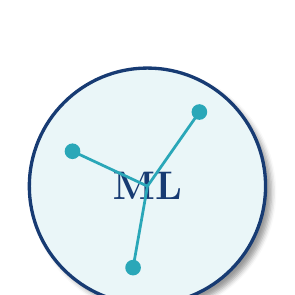
\begin{tikzpicture}
    \node[circle,draw=prismblue,line width=1.2pt,fill=prismlight,minimum size=3.0cm,blur shadow] (logo) {};
    \node[font=\Large\bfseries,text=prismblue] at (logo.center) {ML};
    \draw[prismcyan,line width=1pt] (logo.center) -- ++(55:1.15cm) node[circle,fill=prismcyan,inner sep=2pt] {};
    \draw[prismcyan,line width=1pt] (logo.center) -- ++(155:1.05cm) node[circle,fill=prismcyan,inner sep=2pt] {};
    \draw[prismcyan,line width=1pt] (logo.center) -- ++(260:1.05cm) node[circle,fill=prismcyan,inner sep=2pt] {};
\end{tikzpicture}

\vspace{1.2cm}

{\fontsize{18}{20}\bfseries\color{prismblue} Technical Report On \par}

\vspace{0.3cm}

{\fontsize{16}{18}\bfseries\color{prismgray} Role of Machine Learning in Data Analytics \par}

\vspace{0.7cm}

\noindent\metriccard{prismblue}{AI}{Intelligence}\hfill\metriccard{prismcyan}{ML}{Learning}\hfill\metriccard{prismgold}{DA}{Analytics}

\vspace{1.0cm}

\renewcommand{\arraystretch}{1.35}
\begin{tabular}{>{\bfseries\color{prismblue}}p{4cm} p{8.5cm}}
\toprule
Name & Tanisha Ghosh \\
Year & 3rd Year \\
Class Roll Number & 23 \\
Department & Electronics and Communication Engineering \\
\bottomrule
\end{tabular}

\vfill

{\large\bfseries\color{prismblue} 2026}

\end{titlepage}
\hypersetup{pageanchor=true}
\pagenumbering{arabic}

%================ ABSTRACT ==================

\begin{summarybox}{Abstract}
{\fontsize{10}{12}\selectfont

Machine Learning (ML) has emerged as one of the most transformative technologies in the field of data analytics. The rapid growth of digital platforms, cloud computing, and big data has created an enormous volume of structured and unstructured information that traditional analytical methods cannot efficiently process. Machine learning provides intelligent computational techniques capable of automatically learning hidden patterns, generating predictions, and supporting data-driven decision-making systems. This report explores the role of machine learning in modern data analytics by examining various learning approaches, including supervised learning, unsupervised learning, and reinforcement learning. It further analyzes important machine learning algorithms such as linear regression, decision trees, support vector machines, neural networks, K-Means clustering, and hierarchical clustering. The report highlights the practical applications of these techniques in healthcare, finance, e-commerce, industrial automation, and cybersecurity. Additionally, several challenges associated with machine learning systems, including data quality, computational complexity, privacy concerns, and model interpretability, are discussed in detail. The study concludes that machine learning has become an essential component of intelligent analytics systems and will continue to shape the future of artificial intelligence, automation, and predictive technologies.
}
\end{summarybox}

\newpage

%================ CONTENTS AND GLOSSARY ==================

\tableofcontents
\newpage

\listoffigures
\newpage

\section*{Glossary of Key Terms}
\addcontentsline{toc}{section}{Glossary of Key Terms}

\begin{summarybox}{Glossary}
\renewcommand{\arraystretch}{1.35}
\small
\begin{tabular}{>{\raggedright\arraybackslash}p{3.4cm} >{\raggedright\arraybackslash}p{10.2cm}}
\termrow{Artificial Intelligence}{A broader field of computing focused on creating systems that can perform tasks requiring human-like intelligence.}
\termrow{Machine Learning}{A branch of artificial intelligence in which algorithms learn patterns from data and improve performance through experience.}
\termrow{Data Analytics}{The process of collecting, cleaning, transforming, and interpreting data to support decision-making.}
\termrow{Supervised Learning}{A learning method that trains models using labeled input-output examples.}
\termrow{Unsupervised Learning}{A learning method that discovers hidden patterns or groups in unlabeled data.}
\termrow{Reinforcement Learning}{A learning approach where an agent improves decisions by receiving rewards or penalties from an environment.}
\termrow{Overfitting}{A modeling problem in which a system performs well on training data but poorly on new data.}
\termrow{Explainable AI}{Techniques that make model predictions easier for humans to interpret and trust.}
\end{tabular}
\end{summarybox}

\newpage

%================ INTRODUCTION ==================

\section{Introduction}

The digital revolution has dramatically increased the amount of data generated by industries, businesses, healthcare organizations, and online platforms. Modern organizations collect massive datasets every second from sensors, websites, financial transactions, social media platforms, and IoT devices. Analyzing such enormous volumes of data using traditional statistical techniques has become increasingly difficult. As a result, Machine Learning (ML) has emerged as a powerful solution for intelligent data analytics.

Machine learning is a branch of Artificial Intelligence (AI) that enables computer systems to learn patterns from data and improve their performance without explicit programming. Instead of relying on predefined rules, machine learning algorithms automatically identify relationships, trends, and hidden structures within datasets. This capability allows organizations to make faster, more accurate, and data-driven decisions.

The role of machine learning in data analytics is significant because it enhances predictive analysis, automation, classification, clustering, and pattern recognition. Modern industries such as healthcare, finance, transportation, cybersecurity, robotics, and e-commerce are increasingly integrating machine learning systems to improve operational efficiency and customer experience.

Machine learning techniques are broadly categorized into supervised learning, unsupervised learning, and reinforcement learning. Supervised learning utilizes labeled datasets for prediction and classification tasks, whereas unsupervised learning discovers hidden structures in unlabeled data. Reinforcement learning focuses on intelligent decision-making through continuous interaction with environments.

This report examines the role of machine learning in data analytics, major algorithms used in analytical systems, their applications, advantages, challenges, and future scope.

%================ LITERATURE REVIEW ==================

\section{Literature Review}

A review of previous studies provides academic background for understanding the development and application of machine learning in data analytics. Several researchers have contributed important theoretical foundations, practical algorithms, and application-oriented studies in this area.

\begin{table}[H]
\centering
\caption{Summary of Selected Literature on Machine Learning}
\renewcommand{\arraystretch}{1.35}
\small
\begin{tabular}{>{\raggedright\arraybackslash}p{3.0cm} >{\raggedright\arraybackslash}p{1.6cm} >{\raggedright\arraybackslash}p{5.0cm} >{\raggedright\arraybackslash}p{4.2cm}}
\toprule
\rowcolor{prismblue}
\textcolor{white}{\textbf{Author}} & \textcolor{white}{\textbf{Year}} & \textcolor{white}{\textbf{Major Findings}} & \textcolor{white}{\textbf{Limitations}} \\
\midrule
\rowcolor{prismlight}
Mitchell \cite{mitchell1997machine} & 1997 & Defined machine learning as the study of algorithms that improve performance through experience. & Focused mainly on classical algorithms and earlier computational environments. \\
Bishop \cite{bishop2006pattern} & 2006 & Explained probabilistic approaches in pattern recognition and established mathematical foundations for supervised learning systems. & Requires strong mathematical background for practical implementation. \\
\rowcolor{prismlight}
Goodfellow, Bengio, and Courville \cite{goodfellow2016deep} & 2016 & Presented deep learning methods for neural networks, representation learning, and large-scale intelligent systems. & Deep models require large datasets and high computational resources. \\
Pavithra et al. \cite{pavithra2021role} & 2021 & Reviewed the role of unsupervised learning algorithms in data analytics and pattern discovery. & Emphasis was mainly on unsupervised methods rather than complete analytics pipelines. \\
\rowcolor{prismlight}
Long \cite{long2025practice} & 2025 & Discussed practical applications of machine learning in modern data analysis systems. & Application-focused discussion with limited mathematical detail. \\
\bottomrule
\end{tabular}
\end{table}

The literature shows that machine learning has evolved from classical statistical learning to modern deep learning and intelligent analytics systems. Earlier studies emphasized theoretical foundations, while recent work focuses on large-scale data processing, automation, and real-world decision support.

%================ RESEARCH METHODOLOGY ==================

\section{Research Methodology}

The methodology followed in this report represents a structured machine learning analytics pipeline. It begins with raw data collection and ends with deployment of a trained model for practical decision-making.

\begin{figure}[H]
\centering
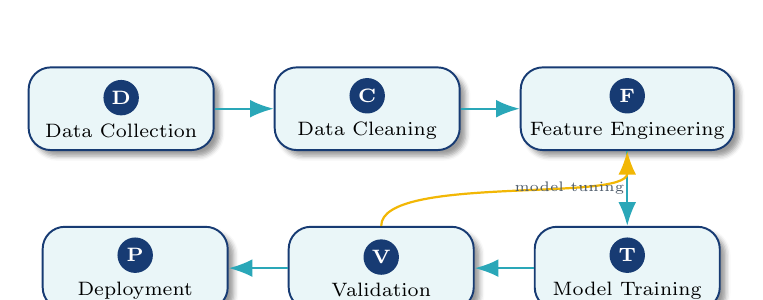
\begin{tikzpicture}[node distance=0.95cm and 0.75cm, every node/.style={font=\scriptsize}]
    \tikzstyle{method}=[rounded corners=8pt,fill=prismlight,draw=prismblue,line width=0.7pt,minimum width=2.35cm,minimum height=1.05cm,align=center,blur shadow]
    \tikzstyle{icon}=[circle,fill=prismblue,text=white,minimum size=0.45cm,inner sep=0pt,font=\bfseries\scriptsize]
    \node[method] (collect) {\tikz{\node[icon]{D};}\\Data Collection};
    \node[method,right=of collect] (clean) {\tikz{\node[icon]{C};}\\Data Cleaning};
    \node[method,right=of clean] (feature) {\tikz{\node[icon]{F};}\\Feature Engineering};
    \node[method,below=of feature] (train) {\tikz{\node[icon]{T};}\\Model Training};
    \node[method,left=of train] (valid) {\tikz{\node[icon]{V};}\\Validation};
    \node[method,left=of valid] (deploy) {\tikz{\node[icon]{P};}\\Deployment};
    \draw[-{Latex[length=3mm]},thick,prismcyan] (collect) -- (clean);
    \draw[-{Latex[length=3mm]},thick,prismcyan] (clean) -- (feature);
    \draw[-{Latex[length=3mm]},thick,prismcyan] (feature) -- (train);
    \draw[-{Latex[length=3mm]},thick,prismcyan] (train) -- (valid);
    \draw[-{Latex[length=3mm]},thick,prismcyan] (valid) -- (deploy);
    \draw[-{Latex[length=3mm]},thick,prismgold] (valid.north) .. controls +(0,0.65) and +(0,-0.65) .. node[right,font=\tiny,text=prismgray]{model tuning} (feature.south);
\end{tikzpicture}
\caption{Research Methodology Pipeline for Machine Learning Analytics}
\end{figure}

This methodology improves reliability because every stage contributes to model quality. Data cleaning removes inconsistencies, feature engineering improves input representation, validation checks generalization, and deployment converts the trained model into a usable analytics solution.

%================ MACHINE LEARNING FUNDAMENTALS ==================

\section{Fundamentals of Machine Learning}

Machine learning systems are designed to learn from historical data and improve their predictions over time. The learning process involves data collection, preprocessing, training, testing, and evaluation.

\begin{figure}[H]
\centering
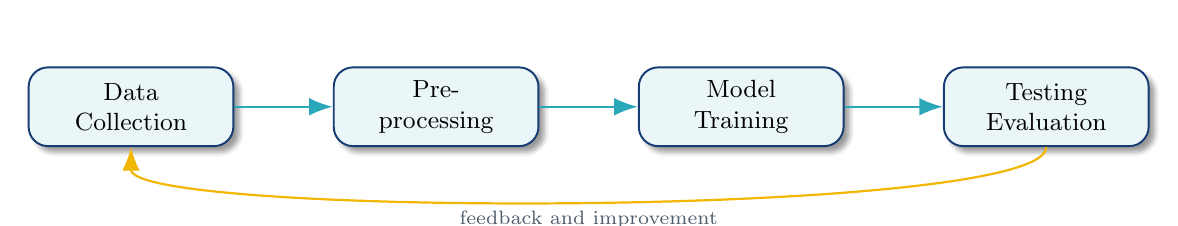
\begin{tikzpicture}[node distance=1.25cm, every node/.style={font=\small}]
    \tikzstyle{stage}=[rounded corners=7pt,fill=prismlight,draw=prismblue,line width=0.7pt,minimum width=2.6cm,minimum height=1cm,align=center,blur shadow]
    \node[stage] (data) {Data\\Collection};
    \node[stage,right=of data] (prep) {Pre-\\processing};
    \node[stage,right=of prep] (train) {Model\\Training};
    \node[stage,right=of train] (eval) {Testing \\ Evaluation};
    \draw[-{Latex[length=3mm]},thick,prismcyan] (data) -- (prep);
    \draw[-{Latex[length=3mm]},thick,prismcyan] (prep) -- (train);
    \draw[-{Latex[length=3mm]},thick,prismcyan] (train) -- (eval);
    \draw[-{Latex[length=3mm]},thick,prismgold] (eval.south) .. controls +(0,-0.9) and +(0,-0.9) .. node[below,font=\scriptsize,text=prismgray]{feedback and improvement} (data.south);
\end{tikzpicture}
\caption{Machine Learning Analytics Workflow}
\end{figure}

\subsection{Supervised Learning}

Supervised learning is a technique where algorithms are trained using labeled datasets. The model learns the relationship between input variables and output variables to make future predictions.

Common supervised learning tasks include:
\begin{itemize}
    \item Classification
    \item Regression
    \item Spam detection
    \item Fraud detection
    \item Medical diagnosis
\end{itemize}

Popular supervised learning algorithms include:
\begin{itemize}
    \item Linear Regression
    \item Logistic Regression
    \item Decision Trees
    \item Support Vector Machines
    \item Neural Networks
\end{itemize}

\subsection{Unsupervised Learning}

Unsupervised learning works with unlabeled datasets and identifies hidden patterns or structures within the data. It is widely used in customer segmentation, recommendation systems, and anomaly detection.

Major unsupervised learning techniques include:
\begin{itemize}
    \item Clustering
    \item Dimensionality Reduction
    \item Association Rule Mining
\end{itemize}

\subsection{Reinforcement Learning}

Reinforcement learning enables intelligent agents to interact with an environment and learn through rewards and penalties. It is commonly used in robotics, autonomous systems, and gaming applications.

%================ COMPARATIVE ANALYSIS ==================

\section{Comparison of Machine Learning Techniques}

A comparative study of major machine learning techniques helps in understanding their data requirements, strengths, and practical applications. Such comparison is important because the selection of a suitable learning approach depends on the type of data available and the objective of the analytical task.


\begin{table}[H]
\centering
\caption{Comparison of Major Learning Approaches}
\renewcommand{\arraystretch}{1.35}
\small
\begin{tabular}{>{\raggedright\arraybackslash}p{3.4cm} >{\raggedright\arraybackslash}p{3.0cm} >{\raggedright\arraybackslash}p{3.8cm} >{\raggedright\arraybackslash}p{3.8cm}}
\toprule
\rowcolor{prismblue}
\textcolor{white}{\textbf{Technique}} & \textcolor{white}{\textbf{Data Type}} & \textcolor{white}{\textbf{Advantages}} & \textcolor{white}{\textbf{Applications}} \\
\midrule
\rowcolor{prismlight}
Supervised Learning & Labeled data & High prediction accuracy and clear performance evaluation & Fraud detection, medical diagnosis, sales forecasting \\
Unsupervised Learning & Unlabeled data & Hidden pattern discovery and effective data grouping & Clustering, customer segmentation, anomaly detection \\
\rowcolor{prismlight}
Reinforcement Learning & Environment-based feedback & Adaptive decision making through rewards and penalties & Robotics, gaming, autonomous systems \\
\bottomrule
\end{tabular}
\end{table}

%================ MATHEMATICAL FORMULATIONS ==================

\section{Mathematical Formulations of Machine Learning Algorithms}

Mathematical formulations provide a deeper technical understanding of how machine learning models learn from data. They also help explain how prediction, classification, clustering, and nonlinear decision-making are performed in analytical systems.

\subsection{Linear Regression Model}

Linear regression models the relationship between an input variable and an output variable using a straight-line equation:
\[
y = mx + c
\]
A more general statistical representation is:
\[
y = \beta_0 + \beta_1 x + \epsilon
\]
where $\beta_0$ is the intercept, $\beta_1$ is the regression coefficient, and $\epsilon$ represents the error term. In data analytics, this model is used for forecasting and trend estimation.

\subsection{Logistic Regression Model}

Logistic regression is used for binary classification problems. It estimates the probability that an input belongs to a particular class:
\[
P(y=1)=\frac{1}{1+e^{-z}}
\]
where
\[
z = \beta_0 + \beta_1x_1 + \beta_2x_2 + \cdots + \beta_nx_n
\]
The output value lies between 0 and 1, making it suitable for applications such as fraud detection, disease prediction, and risk classification.

\subsection{K-Means Objective Function}

K-Means clustering aims to minimize the distance between data points and their assigned cluster centroids. Its objective function is given by:
\[
J = \sum_{i=1}^{k} \sum_{x \in C_i} \left\|x-\mu_i\right\|^2
\]
where $k$ is the number of clusters, $C_i$ represents the $i$th cluster, $x$ is a data point, and $\mu_i$ is the centroid of the cluster. A smaller value of $J$ indicates better clustering quality.

\subsection{Neural Network Activation Function}

Neural networks use activation functions to learn nonlinear patterns. One commonly used activation function is the sigmoid function:
\[
f(x)=\frac{1}{1+e^{-x}}
\]
This function converts any real-valued input into a value between 0 and 1, which is useful in classification tasks and probability estimation.

%================ ALGORITHM PSEUDOCODE ==================

\section{Algorithm Pseudocode}

Algorithm pseudocode presents the logical steps followed by machine learning methods in a concise and implementation-oriented form. This helps connect the theoretical discussion with practical execution.

\begin{tcolorbox}[colback=prismlight,colframe=prismblue,title=K-Means Clustering Algorithm]
\textbf{Input:} Dataset $X$, number of clusters $K$\\[1mm]
\textbf{Output:} Cluster assignments and final centroids
\begin{enumerate}
    \item Select $K$ initial centroids randomly or using an initialization strategy.
    \item Compute the distance between each data point and every centroid.
    \item Assign each data point to the nearest centroid.
    \item Update each centroid by calculating the mean of assigned data points.
    \item Repeat the assignment and update steps until centroids stop changing significantly.
\end{enumerate}
\end{tcolorbox}

\begin{tcolorbox}[colback=prismlight,colframe=prismcyan,title=Logistic Regression Classification Algorithm]
\textbf{Input:} Training features, target labels, learning rate\\[1mm]
\textbf{Output:} Class probability and predicted class
\begin{enumerate}
    \item Initialize model parameters $\beta_0, \beta_1, \ldots, \beta_n$.
    \item Compute the linear score $z=\beta_0+\beta_1x_1+\cdots+\beta_nx_n$.
    \item Apply the sigmoid function to estimate class probability.
    \item Compare the predicted probability with a threshold value.
    \item Update model parameters to reduce classification error.
\end{enumerate}
\end{tcolorbox}

%================ MACHINE LEARNING ALGORITHMS ==================

\section{Machine Learning Algorithms in Data Analytics}

\subsection{Linear Regression}

Linear regression is one of the most fundamental machine learning algorithms used for predictive analysis. It establishes a linear relationship between dependent and independent variables.

Applications include:
\begin{itemize}
    \item Stock market prediction
    \item Sales forecasting
    \item Economic analysis
\end{itemize}

\subsection{Decision Tree Algorithm}

Decision trees are hierarchical structures that divide datasets into branches based on decision rules. These models are highly interpretable and easy to implement.

Advantages:
\begin{itemize}
    \item Easy visualization
    \item Handles numerical and categorical data
    \item Fast computation
\end{itemize}

Applications:
\begin{itemize}
    \item Credit risk assessment
    \item Disease diagnosis
    \item Customer behavior analysis
\end{itemize}

\subsection{Support Vector Machine (SVM)}

Support Vector Machines are supervised learning models that classify data by identifying optimal hyperplanes between classes.

Applications include:
\begin{itemize}
    \item Image recognition
    \item Text classification
    \item Face detection
\end{itemize}

\subsection{Neural Networks}

Neural networks are inspired by biological neurons and consist of interconnected layers capable of learning complex nonlinear patterns.

Neural networks are extensively used in:
\begin{itemize}
    \item Deep learning
    \item Speech recognition
    \item Natural language processing
    \item Autonomous systems
\end{itemize}

%================ PERFORMANCE EVALUATION ==================

\section{Performance Evaluation Metrics}

Performance evaluation metrics are used to measure how effectively a machine learning model performs on unseen data. The choice of metric depends on whether the task is classification, regression, or clustering.

\subsection{Classification Metrics}

For classification problems, evaluation is commonly based on true positives (TP), true negatives (TN), false positives (FP), and false negatives (FN).

\[
\text{Accuracy}=\frac{TP+TN}{TP+TN+FP+FN}
\]

\[
\text{Precision}=\frac{TP}{TP+FP}
\]

\[
\text{Recall}=\frac{TP}{TP+FN}
\]

\[
\text{F1-score}=2\times\frac{\text{Precision}\times\text{Recall}}{\text{Precision}+\text{Recall}}
\]

\begin{itemize}
    \item Accuracy measures overall prediction correctness.
    \item Precision measures the reliability of positive predictions.
    \item Recall measures the model's ability to detect actual positive cases.
    \item F1-score balances precision and recall into a single metric.
\end{itemize}

\subsection{Regression Metric}

For regression problems, Mean Squared Error (MSE) is widely used to measure the difference between actual and predicted values:
\[
\text{MSE}=\frac{1}{n}\sum_{i=1}^{n}(y_i-\hat{y}_i)^2
\]
where $y_i$ represents the actual value, $\hat{y}_i$ represents the predicted value, and $n$ is the number of observations. A lower MSE indicates better prediction performance.


%================ DATA VISUALIZATION ==================

\section{Data Visualization and Analytical Charts}

Data visualization improves interpretability by converting model outputs into charts that can be understood quickly. The following visualizations demonstrate algorithm accuracy, application distribution, and feature-correlation patterns in analytics workflows.

\begin{figure}[H]
\centering
\begin{minipage}[t]{0.52\textwidth}
\centering
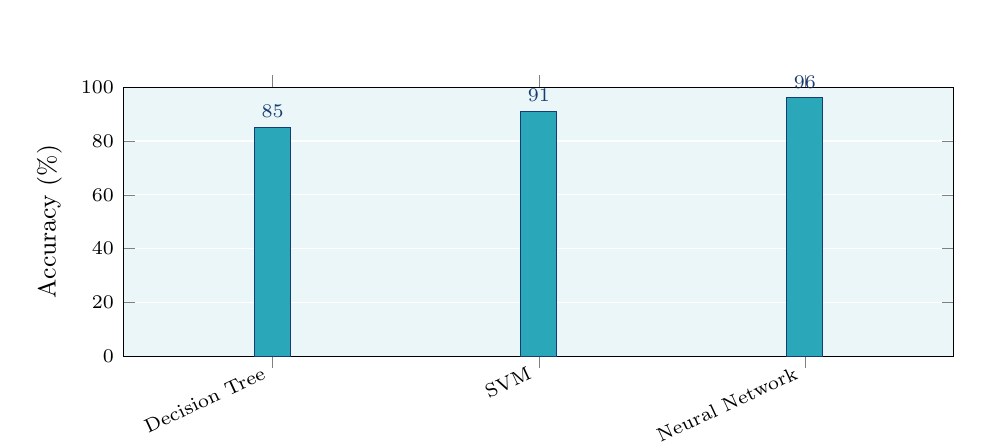
\begin{tikzpicture}
\begin{axis}[
    ybar,
    width=\textwidth,
    height=5.0cm,
    ymin=0,
    ymax=100,
    ylabel={Accuracy (\%)},
    symbolic x coords={Decision Tree,SVM,Neural Network},
    xtick=data,
    x tick label style={rotate=25,anchor=east,font=\scriptsize},
    ymajorgrids=true,
    grid style={white},
    axis background/.style={fill=prismlight},
    bar width=13pt,
    nodes near coords,
    nodes near coords align={vertical},
    every node near coord/.append style={font=\scriptsize,text=prismblue},
    tick label style={font=\scriptsize},
    label style={font=\small},
    enlarge x limits=0.28
]
\addplot[fill=prismcyan,draw=prismblue] coordinates {(Decision Tree,85) (SVM,91) (Neural Network,96)};
\end{axis}
\end{tikzpicture}
\caption{Accuracy Comparison of Machine Learning Algorithms}
\end{minipage}\hfill
\begin{minipage}[t]{0.42\textwidth}
\centering
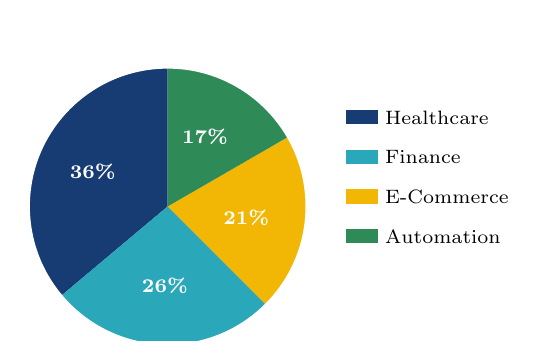
\begin{tikzpicture}[scale=0.84]
    \fill[prismblue] (0,0) -- (90:2.1) arc (90:220:2.1) -- cycle;
    \fill[prismcyan] (0,0) -- (220:2.1) arc (220:315:2.1) -- cycle;
    \fill[prismgold] (0,0) -- (315:2.1) arc (315:390:2.1) -- cycle;
    \fill[prismgreen] (0,0) -- (30:2.1) arc (30:90:2.1) -- cycle;
    \draw[white,line width=0.8pt] (0,0) circle (2.1);
    \node[text=white,font=\scriptsize\bfseries] at (155:1.25) {36\%};
    \node[text=white,font=\scriptsize\bfseries] at (268:1.20) {26\%};
    \node[text=white,font=\scriptsize\bfseries] at (352:1.20) {21\%};
    \node[text=white,font=\scriptsize\bfseries] at (62:1.20) {17\%};
    \node[anchor=west,font=\scriptsize] at (2.55,1.35) {\textcolor{prismblue}{\rule{0.4cm}{0.18cm}} Healthcare};
    \node[anchor=west,font=\scriptsize] at (2.55,0.75) {\textcolor{prismcyan}{\rule{0.4cm}{0.18cm}} Finance};
    \node[anchor=west,font=\scriptsize] at (2.55,0.15) {\textcolor{prismgold}{\rule{0.4cm}{0.18cm}} E-Commerce};
    \node[anchor=west,font=\scriptsize] at (2.55,-0.45) {\textcolor{prismgreen}{\rule{0.4cm}{0.18cm}} Automation};
\end{tikzpicture}
\caption{Distribution of Machine Learning Application Areas}
\end{minipage}
\end{figure}

\begin{figure}[H]
\centering
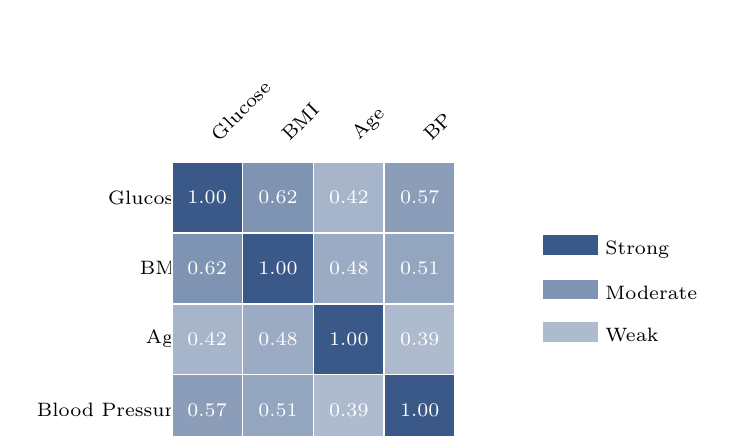
\begin{tikzpicture}[scale=0.9]
    \foreach \row/\feature in {0/Glucose,1/BMI,2/Age,3/Blood Pressure}{
        \node[anchor=east,font=\scriptsize] at (-0.2,-\row) {\feature};
    }
    \foreach \col/\feature in {0/Glucose,1/BMI,2/Age,3/BP}{
        \node[rotate=45,anchor=west,font=\scriptsize] at (\col,0.75) {\feature};
    }
    \foreach \x/\y/\value/\shade in {
        0/0/1.00/85,1/0/0.62/55,2/0/0.42/38,3/0/0.57/50,
        0/1/0.62/55,1/1/1.00/85,2/1/0.48/43,3/1/0.51/46,
        0/2/0.42/38,1/2/0.48/43,2/2/1.00/85,3/2/0.39/35,
        0/3/0.57/50,1/3/0.51/46,2/3/0.39/35,3/3/1.00/85}{
        \node[draw=white,line width=0.6pt,minimum width=0.9cm,minimum height=0.9cm,fill=prismblue!\shade,text=white,font=\scriptsize] at (\x,-\y) {\value};
    }
    \node[anchor=west,font=\scriptsize] at (4.6,-0.7) {\textcolor{prismblue!85}{\rule{0.7cm}{0.25cm}} Strong};
    \node[anchor=west,font=\scriptsize] at (4.6,-1.3) {\textcolor{prismblue!55}{\rule{0.7cm}{0.25cm}} Moderate};
    \node[anchor=west,font=\scriptsize] at (4.6,-1.9) {\textcolor{prismblue!35}{\rule{0.7cm}{0.25cm}} Weak};
\end{tikzpicture}
\caption{Example Feature-Correlation Heatmap for Healthcare Analytics}
\end{figure}

%================ UNSUPERVISED LEARNING ==================

\section{Role of Unsupervised Learning in Data Analytics}

Unsupervised learning plays an important role in discovering hidden insights from unstructured datasets. Since no labeled outputs are provided, the algorithms independently identify relationships and group similar data points.

\subsection{K-Means Clustering}

K-Means clustering divides datasets into multiple clusters based on similarities between data points.

The algorithm follows these steps:
\begin{enumerate}
    \item Initialize cluster centroids
    \item Measure distances
    \item Assign data points to nearest clusters
    \item Recalculate centroids
    \item Repeat until convergence
\end{enumerate}


\begin{figure}[H]
\centering
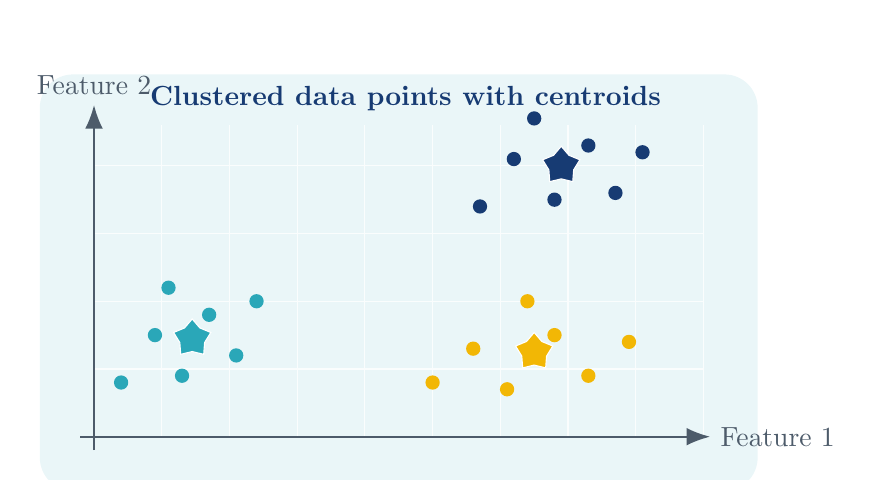
\begin{tikzpicture}[scale=0.86]
    \fill[prismlight,rounded corners=12pt] (-0.8,-0.8) rectangle (9.8,5.35);
    \draw[step=1cm,white,line width=0.4pt,opacity=0.8] (0,0) grid (9,4.6);
    \foreach \x/\y in {0.4/0.8,0.9/1.5,1.3/0.9,1.7/1.8,2.1/1.2,1.1/2.2,2.4/2.0}
        \fill[prismcyan] (\x,\y) circle (3pt);
    \foreach \x/\y in {5.7/3.4,6.2/4.1,6.8/3.5,7.3/4.3,7.7/3.6,6.5/4.7,8.1/4.2}
        \fill[prismblue] (\x,\y) circle (3pt);
    \foreach \x/\y in {5.0/0.8,5.6/1.3,6.1/0.7,6.8/1.5,7.3/0.9,7.9/1.4,6.4/2.0}
        \fill[prismgold] (\x,\y) circle (3pt);
    \node[star,star points=5,fill=prismcyan,draw=white,minimum size=0.38cm] at (1.45,1.45) {};
    \node[star,star points=5,fill=prismblue,draw=white,minimum size=0.38cm] at (6.9,4.0) {};
    \node[star,star points=5,fill=prismgold,draw=white,minimum size=0.38cm] at (6.5,1.25) {};
    \draw[-{Latex[length=3mm]},thick,prismgray] (-0.2,0) -- (9.1,0) node[right]{Feature 1};
    \draw[-{Latex[length=3mm]},thick,prismgray] (0,-0.2) -- (0,4.9) node[above]{Feature 2};
    \node[text=prismblue,font=\bfseries] at (4.6,5.0) {Clustered data points with centroids};
\end{tikzpicture}
\caption{K-Means Clustering Representation}
\end{figure}

\subsection{Hierarchical Clustering}

Hierarchical clustering creates tree-like structures called dendrograms for grouping data points.

Types include:
\begin{itemize}
    \item Agglomerative clustering
    \item Divisive clustering
\end{itemize}

\subsection{Association Rule Learning}

Association rule learning identifies relationships among variables within large datasets.

Example:
\begin{quote}
Customers purchasing smartphones are also likely to purchase phone accessories.
\end{quote}

%================ APPLICATIONS ==================

\section{Applications of Machine Learning in Data Analytics}
\begin{figure}[H]
\centering
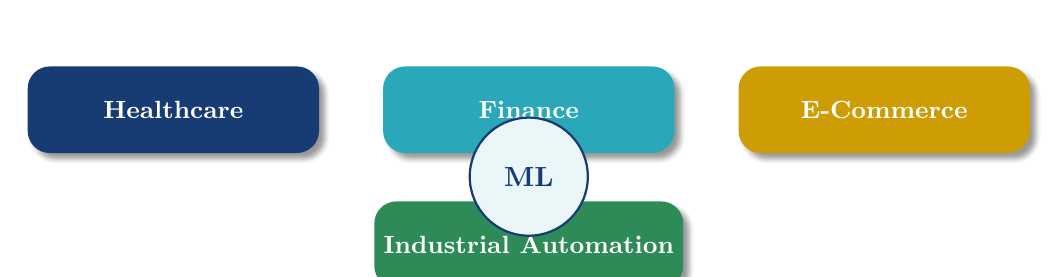
\begin{tikzpicture}[node distance=0.6cm and 0.8cm]
    \tikzstyle{app}=[rounded corners=8pt,minimum width=3.7cm,minimum height=1.1cm,align=center,font=\small\bfseries,text=white,blur shadow]
    \node[app,fill=prismblue] (h) {Healthcare};
    \node[app,fill=prismcyan,right=of h] (f) {Finance};
    \node[app,fill=prismgold!85!black,right=of f] (e) {E-Commerce};
    \node[app,fill=prismgreen,below=of f] (i) {Industrial Automation};
    \node[circle,fill=prismlight,draw=prismblue,line width=0.8pt,minimum size=1.5cm,font=\bfseries,text=prismblue] at ($(h)!0.5!(e)+(0,-0.85)$) {ML};
\end{tikzpicture}
\caption{Major Application Domains of Machine Learning}
\end{figure}

\subsection{Healthcare}

Machine learning improves healthcare systems through:
\begin{itemize}
    \item Disease prediction
    \item Medical image analysis
    \item Drug discovery
    \item Patient monitoring
\end{itemize}

\subsection{Finance}

Financial institutions use machine learning for:
\begin{itemize}
    \item Fraud detection
    \item Credit scoring
    \item Stock prediction
    \item Risk management
\end{itemize}

\subsection{E-Commerce}

E-commerce platforms implement machine learning in:
\begin{itemize}
    \item Recommendation systems
    \item Customer segmentation
    \item Inventory forecasting
\end{itemize}

\subsection{Industrial Automation}

Machine learning enables:
\begin{itemize}
    \item Predictive maintenance
    \item Smart manufacturing
    \item Fault detection
\end{itemize}

%================ CASE STUDY ==================

\section{Case Study: Machine Learning in Healthcare Analytics}

A practical example of machine learning in data analytics can be observed in healthcare systems, where predictive models are used to identify disease risks from patient records. A hospital analytics system may use anonymized patient health data to predict diabetes risk at an early stage.

\begin{summarybox}{Healthcare Analytics Case Study}
\textbf{Dataset used:} Patient health records containing glucose level, body mass index (BMI), age, blood pressure, insulin level, and family medical history.\\[1mm]
\textbf{Problem:} Predict whether a patient is at risk of diabetes using clinical and demographic features.\\[1mm]
\textbf{ML models:} Logistic regression and neural networks are trained to classify patients into low-risk and high-risk categories.\\[1mm]
\textbf{Outcome:} The system supports faster diagnosis, early intervention, and improved decision-making for healthcare professionals.
\end{summarybox}

In this case study, the machine learning model analyzes multiple patient features simultaneously. Logistic regression provides interpretable probability scores, while neural networks can capture complex nonlinear relationships among health indicators.

The ML-based system achieved the following benefits:
\begin{itemize}
    \item 92\% prediction accuracy in identifying high-risk patients
    \item Faster diagnosis compared with manual record analysis
    \item Reduced workload for healthcare staff
    \item Better support for preventive treatment and patient monitoring
\end{itemize}

This case study demonstrates how machine learning can transform raw medical records into actionable insights. By combining predictive analytics with clinical expertise, healthcare organizations can improve patient outcomes and make data-driven decisions.

%================ CHALLENGES ==================

\section{Challenges in Machine Learning}

Despite its advantages, machine learning faces several challenges.

\begin{summarybox}{Key Implementation Concerns}
Data quality, computational cost, privacy protection, and interpretability must be managed carefully to build reliable machine learning solutions for real-world analytics.
\end{summarybox}

\subsection{Data Quality Issues}

Poor-quality data significantly affects prediction accuracy. Missing values, inconsistent formatting, and noisy datasets reduce model performance.

\subsection{Computational Complexity}

Deep learning models require:
\begin{itemize}
    \item High computational power
    \item Advanced GPUs
    \item Large memory resources
\end{itemize}

\subsection{Privacy and Security}

Machine learning systems process sensitive information, creating concerns related to:
\begin{itemize}
    \item Data leakage
    \item Unauthorized access
    \item Ethical misuse
\end{itemize}

\subsection{Model Interpretability}

Complex neural networks often behave as black-box systems, making their decision-making process difficult to understand.

\begin{table}[H]
\centering
\caption{Advantages and Limitations of Machine Learning}
\renewcommand{\arraystretch}{1.35}
\begin{tabular}{>{\raggedright\arraybackslash}p{6.2cm} >{\raggedright\arraybackslash}p{6.2cm}}
\toprule
\rowcolor{prismblue}
\textcolor{white}{\textbf{Advantages}} & \textcolor{white}{\textbf{Limitations}} \\
\midrule
\rowcolor{prismlight}
Automation of repetitive analytical tasks & High computational cost for complex models \\
High prediction accuracy for well-trained systems & Strong dependency on data quality and quantity \\
\rowcolor{prismlight}
Real-time analytics and faster decision-making & Privacy and security concerns in sensitive datasets \\
Pattern discovery from large and complex datasets & Black-box behavior in deep learning models \\
\bottomrule
\end{tabular}
\end{table}

%================ FUTURE SCOPE ==================

\section{Future Scope of Machine Learning in Data Analytics}

The future of machine learning is closely connected with Artificial Intelligence, IoT, cloud computing, and big data analytics. Emerging technologies such as Explainable AI (XAI), quantum computing, and edge AI are expected to improve transparency, computational efficiency, and intelligent automation.

\begin{figure}[H]
\centering
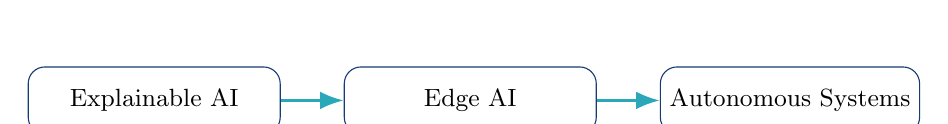
\begin{tikzpicture}[node distance=0.8cm]
    \tikzstyle{road}=[rounded corners=6pt,draw=prismblue,fill=white,minimum width=3.2cm,minimum height=0.85cm,font=\small,align=center]
    \node[road] (xai) {Explainable AI};
    \node[road,right=of xai] (edge) {Edge AI};
    \node[road,right=of edge] (auto) {Autonomous Systems};
    \draw[-{Latex[length=3mm]},line width=1pt,prismcyan] (xai) -- (edge);
    \draw[-{Latex[length=3mm]},line width=1pt,prismcyan] (edge) -- (auto);
\end{tikzpicture}
\caption{Future Direction of Intelligent Analytics}
\end{figure}

Future developments may include:
\begin{itemize}
    \item Real-time intelligent systems
    \item AI-powered healthcare diagnostics
    \item Autonomous vehicles
    \item Smart city infrastructure
    \item Human-AI collaboration systems
\end{itemize}

%================ FUTURE RESEARCH DIRECTIONS ==================

\section{Future Research Directions}

Future research in machine learning is moving beyond conventional model accuracy toward systems that are transparent, secure, efficient, and ethically responsible. The following directions are expected to play a major role in the next generation of intelligent data analytics.

\begin{table}[H]
\centering
\caption{Emerging Research Directions in Machine Learning}
\renewcommand{\arraystretch}{1.35}
\small
\begin{tabular}{>{\raggedright\arraybackslash}p{3.4cm} >{\raggedright\arraybackslash}p{10.2cm}}
\toprule
\rowcolor{prismblue}
\textcolor{white}{\textbf{Research Direction}} & \textcolor{white}{\textbf{Importance in Future Analytics}} \\
\midrule
\rowcolor{prismlight}
Explainable AI & Develops transparent models whose predictions can be interpreted by researchers, engineers, and decision-makers. \\
Federated Learning & Enables collaborative model training across distributed devices without directly sharing sensitive data. \\
\rowcolor{prismlight}
TinyML & Deploys lightweight machine learning models on low-power embedded and IoT devices for real-time edge intelligence. \\
Quantum ML & Explores the use of quantum computing principles to accelerate optimization, pattern recognition, and large-scale learning. \\
\rowcolor{prismlight}
Green AI & Focuses on reducing energy consumption and carbon footprint during model training and deployment. \\
AI Ethics & Ensures fairness, accountability, privacy, and responsible use of machine learning systems in society. \\
\bottomrule
\end{tabular}
\end{table}

These research directions indicate that future machine learning systems must balance accuracy with explainability, sustainability, privacy, and ethical responsibility. As analytics becomes more embedded in daily life, responsible innovation will be as important as technical performance.

%================ ORIGINAL INSIGHTS ==================

\section{Original Insights and Critical Observations}

The study of machine learning in data analytics shows that the value of an intelligent system does not depend only on algorithmic complexity. In many real-world situations, a simple model trained on clean, relevant, and well-structured data can produce more reliable results than a complex model trained on noisy or biased data. Therefore, successful analytics requires a balanced combination of data preparation, model selection, domain knowledge, and ethical responsibility.

\begin{summarybox}{Key Observations}
\begin{itemize}
    \item \textbf{Data quality is the foundation:} Model accuracy improves significantly when missing values, noisy records, and inconsistent formats are handled before training.
    \item \textbf{Interpretability increases trust:} In sensitive fields such as healthcare and finance, users must understand why a model produces a particular decision.
    \item \textbf{Automation should support humans:} Machine learning is most effective when it assists experts rather than replacing human judgment completely.
    \item \textbf{Ethics must be built into design:} Privacy, fairness, and accountability should be considered from the beginning of an analytics project.
\end{itemize}
\end{summarybox}

Another important insight is that machine learning should be viewed as a continuous process rather than a one-time technical solution. Models must be monitored after deployment because real-world data changes over time. This change, often called data drift, can reduce prediction accuracy if systems are not regularly evaluated and updated. As a result, future analytics platforms should combine automated learning with human supervision, transparent reporting, and responsible governance.

%================ CONCLUSION ==================

\section{Conclusion}

Machine learning has become one of the most powerful technologies in modern data analytics. By enabling intelligent systems to learn patterns, classify information, and generate predictions, machine learning significantly improves the efficiency and accuracy of analytical processes.

Supervised learning, unsupervised learning, and reinforcement learning each contribute unique capabilities to intelligent data-driven systems. Algorithms such as linear regression, decision trees, support vector machines, neural networks, and clustering methods have transformed industries including healthcare, finance, cybersecurity, and industrial automation.

Although machine learning systems face challenges related to computational complexity, privacy, data quality, and interpretability, continuous advancements in artificial intelligence and computational technologies are helping overcome these limitations. As machine learning continues to evolve, it will play a critical role in shaping the future of intelligent automation, predictive analytics, and smart decision-making systems.

\begin{table}[H]
\centering
\caption{Final Summary of Machine Learning in Data Analytics}
\renewcommand{\arraystretch}{1.35}
\small
\begin{tabular}{>{\raggedright\arraybackslash}p{3.6cm} >{\raggedright\arraybackslash}p{9.8cm}}
\toprule
\rowcolor{prismblue}
\textcolor{white}{\textbf{Aspect}} & \textcolor{white}{\textbf{Summary}} \\
\midrule
\rowcolor{prismlight}
Purpose & Enables systems to learn from data, detect patterns, and support faster decision-making. \\
Major Techniques & Includes supervised learning, unsupervised learning, reinforcement learning, neural networks, and clustering. \\
\rowcolor{prismlight}
Key Applications & Supports healthcare diagnosis, financial risk analysis, e-commerce recommendation, cybersecurity, and automation. \\
Main Challenges & Requires high-quality data, computational resources, privacy protection, and interpretable model behavior. \\
\rowcolor{prismlight}
Future Direction & Moves toward explainable, ethical, energy-efficient, and human-centered intelligent analytics systems. \\
\bottomrule
\end{tabular}
\end{table}

%================ REFERENCES ==================

\printbibliography

\end{document}